\documentclass[12pt]{article}
\usepackage[letterpaper,top=0.9in,bottom=0.85in,left=0.75in,right=0.75in,
  headheight=16pt,headsep=0.25in,footskip=0.45in]{geometry}
\usepackage[T1]{fontenc}
\usepackage{tgheros}
\renewcommand{\familydefault}{\sfdefault}
\usepackage{tikz}
\usetikzlibrary{arrows.meta,calc}
\usepackage{fancyhdr}
\pagestyle{fancy}
\fancyhf{}
\fancyhead[L]{Week NN / Hidden armies / Grades 2--3}
\fancyfoot[L]{\small Bellingham Math Circle / Week NN / HA-23-v1}
\fancyfoot[R]{\small \thepage}
\renewcommand{\headrulewidth}{0.4pt}
\setlength{\parindent}{0pt}
\setlength{\parskip}{0pt}
\hyphenpenalty=10000
\exhyphenpenalty=10000
\newcommand{\prob}[1]{\par\vspace{16pt}\noindent\textbf{Problem #1:}\ }
\tikzset{sbox/.style={draw,line width=0.6pt,minimum width=#1,minimum height=0.5cm,
  inner sep=0pt,outer sep=0pt,font=\sffamily},sbox/.default=0.56cm}
% a plan strip written inline: cubes on hills 1, 2, 3
\newcommand{\strip}[4][0.56cm]{\hspace{1.5pt}\tikz[baseline={([yshift=-0.75ex]a.center)}]{%
  \node[sbox=#1] (a) {#2};\node[sbox=#1,anchor=west] (b) at (a.east) {#3};%
  \node[sbox=#1,anchor=west] (c) at (b.east) {#4};}\hspace{1.5pt}}
\begin{document}
\raggedright

\begin{minipage}[c]{0.55\linewidth}\raggedright Both players have the same number of cubes. Behind your folder, put all your cubes on the three hills of your mat. This is your plan. A hill can stay empty. Lift the folders at the same time. On each hill, the player with more cubes wins the hill and puts a token on it. If the cubes are equal, nobody wins that hill. The player who wins more hills wins the game. If both players win the same number of hills, the game is a tie. A plan is written as three numbers in a strip: the cubes on hills 1, 2 and 3.\end{minipage}\hfill\begin{minipage}[c]{0.42\linewidth}\centering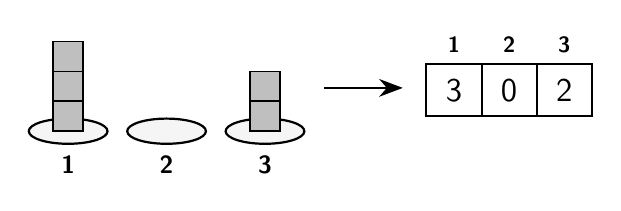
\begin{tikzpicture}[]
\draw[line width=0.8pt,fill=black!4] (0.000,0.000) ellipse (0.5 and 0.16);
\node[font=\small\bfseries] at (0.000,-0.430) {1};
\draw[line width=0.6pt,fill=black!25] (-0.190,0.000) rectangle (0.190,0.380);
\draw[line width=0.6pt,fill=black!25] (-0.190,0.380) rectangle (0.190,0.760);
\draw[line width=0.6pt,fill=black!25] (-0.190,0.760) rectangle (0.190,1.140);
\draw[line width=0.8pt,fill=black!4] (1.250,0.000) ellipse (0.5 and 0.16);
\node[font=\small\bfseries] at (1.250,-0.430) {2};
\draw[line width=0.8pt,fill=black!4] (2.500,0.000) ellipse (0.5 and 0.16);
\node[font=\small\bfseries] at (2.500,-0.430) {3};
\draw[line width=0.6pt,fill=black!25] (2.310,0.000) rectangle (2.690,0.380);
\draw[line width=0.6pt,fill=black!25] (2.310,0.380) rectangle (2.690,0.760);
\draw[-{Stealth[length=3mm]},line width=0.9pt] (3.25,0.55) -- (4.25,0.55);
\draw[line width=0.7pt] (4.550,0.190) rectangle (5.250,0.850);
\node[font=\large] at (4.900,0.520) {3};
\node[font=\footnotesize\bfseries] at (4.900,1.100) {1};
\draw[line width=0.7pt] (5.250,0.190) rectangle (5.950,0.850);
\node[font=\large] at (5.600,0.520) {0};
\node[font=\footnotesize\bfseries] at (5.600,1.100) {2};
\draw[line width=0.7pt] (5.950,0.190) rectangle (6.650,0.850);
\node[font=\large] at (6.300,0.520) {2};
\node[font=\footnotesize\bfseries] at (6.300,1.100) {3};
\end{tikzpicture}\end{minipage}

\prob{1}Play the game with 6 cubes each. For each game, write both plans and circle the plan that won, if one did.
\par\vspace{10pt}\noindent\hspace*{0.3cm}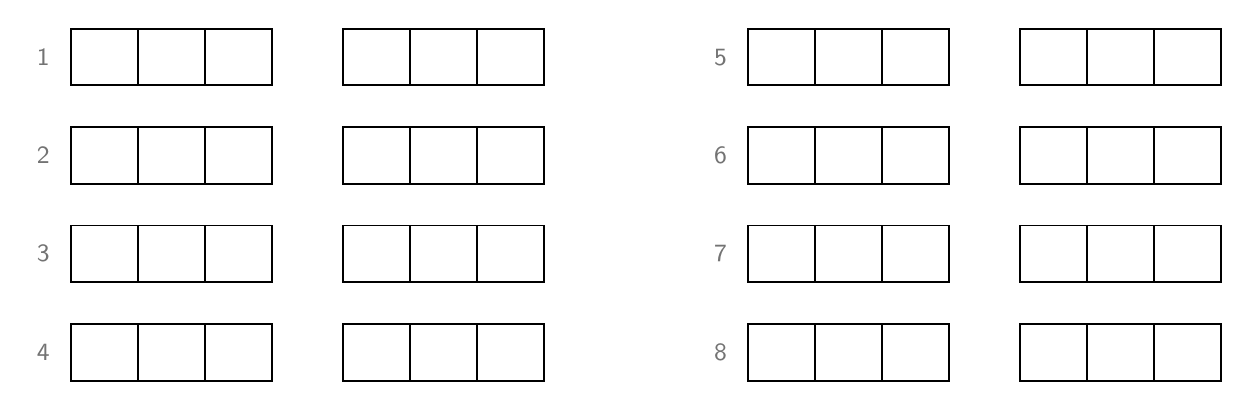
\begin{tikzpicture}[]
\node[font=\small,text=black!55,anchor=east] at (0.350,0.360) {1};
\draw[line width=0.7pt] (0.500,0.000) rectangle (1.350,0.720);
\draw[line width=0.7pt] (1.350,0.000) rectangle (2.200,0.720);
\draw[line width=0.7pt] (2.200,0.000) rectangle (3.050,0.720);
\draw[line width=0.7pt] (3.950,0.000) rectangle (4.800,0.720);
\draw[line width=0.7pt] (4.800,0.000) rectangle (5.650,0.720);
\draw[line width=0.7pt] (5.650,0.000) rectangle (6.500,0.720);
\node[font=\small,text=black!55,anchor=east] at (0.350,-0.890) {2};
\draw[line width=0.7pt] (0.500,-1.250) rectangle (1.350,-0.530);
\draw[line width=0.7pt] (1.350,-1.250) rectangle (2.200,-0.530);
\draw[line width=0.7pt] (2.200,-1.250) rectangle (3.050,-0.530);
\draw[line width=0.7pt] (3.950,-1.250) rectangle (4.800,-0.530);
\draw[line width=0.7pt] (4.800,-1.250) rectangle (5.650,-0.530);
\draw[line width=0.7pt] (5.650,-1.250) rectangle (6.500,-0.530);
\node[font=\small,text=black!55,anchor=east] at (0.350,-2.140) {3};
\draw[line width=0.7pt] (0.500,-2.500) rectangle (1.350,-1.780);
\draw[line width=0.7pt] (1.350,-2.500) rectangle (2.200,-1.780);
\draw[line width=0.7pt] (2.200,-2.500) rectangle (3.050,-1.780);
\draw[line width=0.7pt] (3.950,-2.500) rectangle (4.800,-1.780);
\draw[line width=0.7pt] (4.800,-2.500) rectangle (5.650,-1.780);
\draw[line width=0.7pt] (5.650,-2.500) rectangle (6.500,-1.780);
\node[font=\small,text=black!55,anchor=east] at (0.350,-3.390) {4};
\draw[line width=0.7pt] (0.500,-3.750) rectangle (1.350,-3.030);
\draw[line width=0.7pt] (1.350,-3.750) rectangle (2.200,-3.030);
\draw[line width=0.7pt] (2.200,-3.750) rectangle (3.050,-3.030);
\draw[line width=0.7pt] (3.950,-3.750) rectangle (4.800,-3.030);
\draw[line width=0.7pt] (4.800,-3.750) rectangle (5.650,-3.030);
\draw[line width=0.7pt] (5.650,-3.750) rectangle (6.500,-3.030);
\node[font=\small,text=black!55,anchor=east] at (8.950,0.360) {5};
\draw[line width=0.7pt] (9.100,0.000) rectangle (9.950,0.720);
\draw[line width=0.7pt] (9.950,0.000) rectangle (10.800,0.720);
\draw[line width=0.7pt] (10.800,0.000) rectangle (11.650,0.720);
\draw[line width=0.7pt] (12.550,0.000) rectangle (13.400,0.720);
\draw[line width=0.7pt] (13.400,0.000) rectangle (14.250,0.720);
\draw[line width=0.7pt] (14.250,0.000) rectangle (15.100,0.720);
\node[font=\small,text=black!55,anchor=east] at (8.950,-0.890) {6};
\draw[line width=0.7pt] (9.100,-1.250) rectangle (9.950,-0.530);
\draw[line width=0.7pt] (9.950,-1.250) rectangle (10.800,-0.530);
\draw[line width=0.7pt] (10.800,-1.250) rectangle (11.650,-0.530);
\draw[line width=0.7pt] (12.550,-1.250) rectangle (13.400,-0.530);
\draw[line width=0.7pt] (13.400,-1.250) rectangle (14.250,-0.530);
\draw[line width=0.7pt] (14.250,-1.250) rectangle (15.100,-0.530);
\node[font=\small,text=black!55,anchor=east] at (8.950,-2.140) {7};
\draw[line width=0.7pt] (9.100,-2.500) rectangle (9.950,-1.780);
\draw[line width=0.7pt] (9.950,-2.500) rectangle (10.800,-1.780);
\draw[line width=0.7pt] (10.800,-2.500) rectangle (11.650,-1.780);
\draw[line width=0.7pt] (12.550,-2.500) rectangle (13.400,-1.780);
\draw[line width=0.7pt] (13.400,-2.500) rectangle (14.250,-1.780);
\draw[line width=0.7pt] (14.250,-2.500) rectangle (15.100,-1.780);
\node[font=\small,text=black!55,anchor=east] at (8.950,-3.390) {8};
\draw[line width=0.7pt] (9.100,-3.750) rectangle (9.950,-3.030);
\draw[line width=0.7pt] (9.950,-3.750) rectangle (10.800,-3.030);
\draw[line width=0.7pt] (10.800,-3.750) rectangle (11.650,-3.030);
\draw[line width=0.7pt] (12.550,-3.750) rectangle (13.400,-3.030);
\draw[line width=0.7pt] (13.400,-3.750) rectangle (14.250,-3.030);
\draw[line width=0.7pt] (14.250,-3.750) rectangle (15.100,-3.030);
\end{tikzpicture}
\prob{2}Is there a plan with 6 cubes that nobody can beat? Take turns: one player shows a plan, and the other tries to beat it.
\par\vspace{12pt}\noindent\hspace*{0.3cm}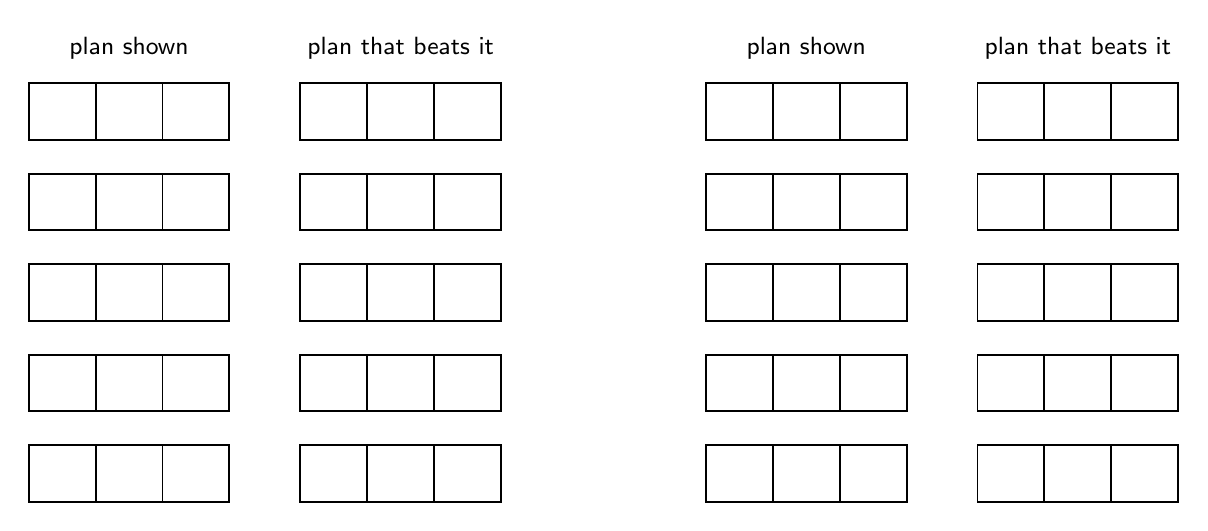
\begin{tikzpicture}[]
\node[font=\small,anchor=south] at (1.775,0.05) {plan shown};
\node[font=\small,anchor=south] at (5.225,0.05) {plan that beats it};
\draw[line width=0.7pt] (0.500,-0.850) rectangle (1.350,-0.130);
\draw[line width=0.7pt] (1.350,-0.850) rectangle (2.200,-0.130);
\draw[line width=0.7pt] (2.200,-0.850) rectangle (3.050,-0.130);
\draw[line width=0.7pt] (3.950,-0.850) rectangle (4.800,-0.130);
\draw[line width=0.7pt] (4.800,-0.850) rectangle (5.650,-0.130);
\draw[line width=0.7pt] (5.650,-0.850) rectangle (6.500,-0.130);
\draw[line width=0.7pt] (0.500,-2.000) rectangle (1.350,-1.280);
\draw[line width=0.7pt] (1.350,-2.000) rectangle (2.200,-1.280);
\draw[line width=0.7pt] (2.200,-2.000) rectangle (3.050,-1.280);
\draw[line width=0.7pt] (3.950,-2.000) rectangle (4.800,-1.280);
\draw[line width=0.7pt] (4.800,-2.000) rectangle (5.650,-1.280);
\draw[line width=0.7pt] (5.650,-2.000) rectangle (6.500,-1.280);
\draw[line width=0.7pt] (0.500,-3.150) rectangle (1.350,-2.430);
\draw[line width=0.7pt] (1.350,-3.150) rectangle (2.200,-2.430);
\draw[line width=0.7pt] (2.200,-3.150) rectangle (3.050,-2.430);
\draw[line width=0.7pt] (3.950,-3.150) rectangle (4.800,-2.430);
\draw[line width=0.7pt] (4.800,-3.150) rectangle (5.650,-2.430);
\draw[line width=0.7pt] (5.650,-3.150) rectangle (6.500,-2.430);
\draw[line width=0.7pt] (0.500,-4.300) rectangle (1.350,-3.580);
\draw[line width=0.7pt] (1.350,-4.300) rectangle (2.200,-3.580);
\draw[line width=0.7pt] (2.200,-4.300) rectangle (3.050,-3.580);
\draw[line width=0.7pt] (3.950,-4.300) rectangle (4.800,-3.580);
\draw[line width=0.7pt] (4.800,-4.300) rectangle (5.650,-3.580);
\draw[line width=0.7pt] (5.650,-4.300) rectangle (6.500,-3.580);
\draw[line width=0.7pt] (0.500,-5.450) rectangle (1.350,-4.730);
\draw[line width=0.7pt] (1.350,-5.450) rectangle (2.200,-4.730);
\draw[line width=0.7pt] (2.200,-5.450) rectangle (3.050,-4.730);
\draw[line width=0.7pt] (3.950,-5.450) rectangle (4.800,-4.730);
\draw[line width=0.7pt] (4.800,-5.450) rectangle (5.650,-4.730);
\draw[line width=0.7pt] (5.650,-5.450) rectangle (6.500,-4.730);
\node[font=\small,anchor=south] at (10.375,0.05) {plan shown};
\node[font=\small,anchor=south] at (13.825,0.05) {plan that beats it};
\draw[line width=0.7pt] (9.100,-0.850) rectangle (9.950,-0.130);
\draw[line width=0.7pt] (9.950,-0.850) rectangle (10.800,-0.130);
\draw[line width=0.7pt] (10.800,-0.850) rectangle (11.650,-0.130);
\draw[line width=0.7pt] (12.550,-0.850) rectangle (13.400,-0.130);
\draw[line width=0.7pt] (13.400,-0.850) rectangle (14.250,-0.130);
\draw[line width=0.7pt] (14.250,-0.850) rectangle (15.100,-0.130);
\draw[line width=0.7pt] (9.100,-2.000) rectangle (9.950,-1.280);
\draw[line width=0.7pt] (9.950,-2.000) rectangle (10.800,-1.280);
\draw[line width=0.7pt] (10.800,-2.000) rectangle (11.650,-1.280);
\draw[line width=0.7pt] (12.550,-2.000) rectangle (13.400,-1.280);
\draw[line width=0.7pt] (13.400,-2.000) rectangle (14.250,-1.280);
\draw[line width=0.7pt] (14.250,-2.000) rectangle (15.100,-1.280);
\draw[line width=0.7pt] (9.100,-3.150) rectangle (9.950,-2.430);
\draw[line width=0.7pt] (9.950,-3.150) rectangle (10.800,-2.430);
\draw[line width=0.7pt] (10.800,-3.150) rectangle (11.650,-2.430);
\draw[line width=0.7pt] (12.550,-3.150) rectangle (13.400,-2.430);
\draw[line width=0.7pt] (13.400,-3.150) rectangle (14.250,-2.430);
\draw[line width=0.7pt] (14.250,-3.150) rectangle (15.100,-2.430);
\draw[line width=0.7pt] (9.100,-4.300) rectangle (9.950,-3.580);
\draw[line width=0.7pt] (9.950,-4.300) rectangle (10.800,-3.580);
\draw[line width=0.7pt] (10.800,-4.300) rectangle (11.650,-3.580);
\draw[line width=0.7pt] (12.550,-4.300) rectangle (13.400,-3.580);
\draw[line width=0.7pt] (13.400,-4.300) rectangle (14.250,-3.580);
\draw[line width=0.7pt] (14.250,-4.300) rectangle (15.100,-3.580);
\draw[line width=0.7pt] (9.100,-5.450) rectangle (9.950,-4.730);
\draw[line width=0.7pt] (9.950,-5.450) rectangle (10.800,-4.730);
\draw[line width=0.7pt] (10.800,-5.450) rectangle (11.650,-4.730);
\draw[line width=0.7pt] (12.550,-5.450) rectangle (13.400,-4.730);
\draw[line width=0.7pt] (13.400,-5.450) rectangle (14.250,-4.730);
\draw[line width=0.7pt] (14.250,-5.450) rectangle (15.100,-4.730);
\end{tikzpicture}
\newpage
\prob{3}Beat each plan below. Then explain how you can beat any plan with 6 or more cubes that your partner names.
\par\vspace{12pt}\noindent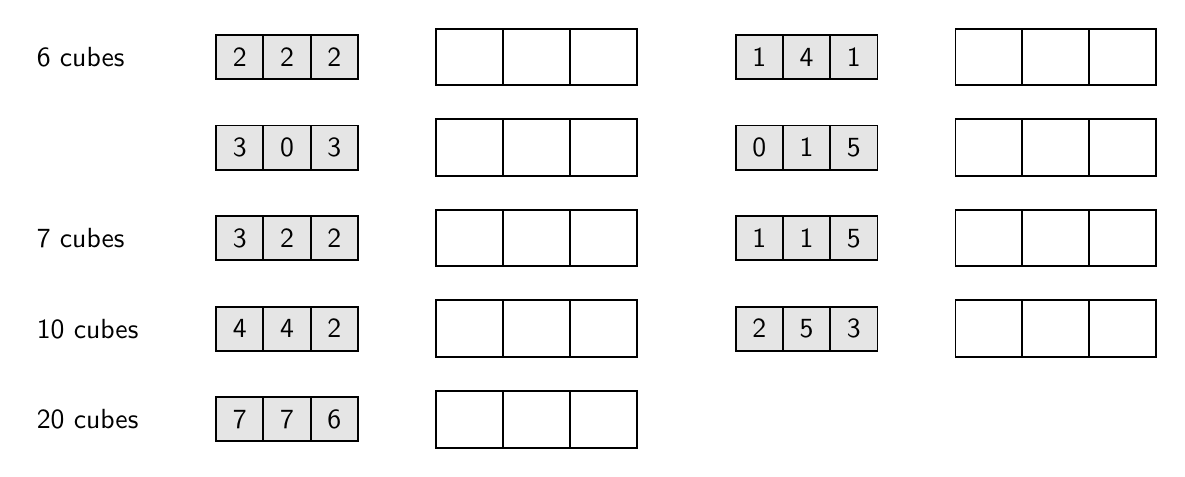
\begin{tikzpicture}[]
\node[anchor=west,font=\normalsize] at (0,0.360) {6 cubes};
\draw[line width=0.7pt,fill=black!10] (2.400,0.080) rectangle (3.000,0.640);
\node[font=\normalsize] at (2.700,0.360) {2};
\draw[line width=0.7pt,fill=black!10] (3.000,0.080) rectangle (3.600,0.640);
\node[font=\normalsize] at (3.300,0.360) {2};
\draw[line width=0.7pt,fill=black!10] (3.600,0.080) rectangle (4.200,0.640);
\node[font=\normalsize] at (3.900,0.360) {2};
\draw[line width=0.7pt] (5.190,0.000) rectangle (6.040,0.720);
\draw[line width=0.7pt] (6.040,0.000) rectangle (6.890,0.720);
\draw[line width=0.7pt] (6.890,0.000) rectangle (7.740,0.720);
\draw[line width=0.7pt,fill=black!10] (9.000,0.080) rectangle (9.600,0.640);
\node[font=\normalsize] at (9.300,0.360) {1};
\draw[line width=0.7pt,fill=black!10] (9.600,0.080) rectangle (10.200,0.640);
\node[font=\normalsize] at (9.900,0.360) {4};
\draw[line width=0.7pt,fill=black!10] (10.200,0.080) rectangle (10.800,0.640);
\node[font=\normalsize] at (10.500,0.360) {1};
\draw[line width=0.7pt] (11.790,0.000) rectangle (12.640,0.720);
\draw[line width=0.7pt] (12.640,0.000) rectangle (13.490,0.720);
\draw[line width=0.7pt] (13.490,0.000) rectangle (14.340,0.720);
\draw[line width=0.7pt,fill=black!10] (2.400,-1.070) rectangle (3.000,-0.510);
\node[font=\normalsize] at (2.700,-0.790) {3};
\draw[line width=0.7pt,fill=black!10] (3.000,-1.070) rectangle (3.600,-0.510);
\node[font=\normalsize] at (3.300,-0.790) {0};
\draw[line width=0.7pt,fill=black!10] (3.600,-1.070) rectangle (4.200,-0.510);
\node[font=\normalsize] at (3.900,-0.790) {3};
\draw[line width=0.7pt] (5.190,-1.150) rectangle (6.040,-0.430);
\draw[line width=0.7pt] (6.040,-1.150) rectangle (6.890,-0.430);
\draw[line width=0.7pt] (6.890,-1.150) rectangle (7.740,-0.430);
\draw[line width=0.7pt,fill=black!10] (9.000,-1.070) rectangle (9.600,-0.510);
\node[font=\normalsize] at (9.300,-0.790) {0};
\draw[line width=0.7pt,fill=black!10] (9.600,-1.070) rectangle (10.200,-0.510);
\node[font=\normalsize] at (9.900,-0.790) {1};
\draw[line width=0.7pt,fill=black!10] (10.200,-1.070) rectangle (10.800,-0.510);
\node[font=\normalsize] at (10.500,-0.790) {5};
\draw[line width=0.7pt] (11.790,-1.150) rectangle (12.640,-0.430);
\draw[line width=0.7pt] (12.640,-1.150) rectangle (13.490,-0.430);
\draw[line width=0.7pt] (13.490,-1.150) rectangle (14.340,-0.430);
\node[anchor=west,font=\normalsize] at (0,-1.940) {7 cubes};
\draw[line width=0.7pt,fill=black!10] (2.400,-2.220) rectangle (3.000,-1.660);
\node[font=\normalsize] at (2.700,-1.940) {3};
\draw[line width=0.7pt,fill=black!10] (3.000,-2.220) rectangle (3.600,-1.660);
\node[font=\normalsize] at (3.300,-1.940) {2};
\draw[line width=0.7pt,fill=black!10] (3.600,-2.220) rectangle (4.200,-1.660);
\node[font=\normalsize] at (3.900,-1.940) {2};
\draw[line width=0.7pt] (5.190,-2.300) rectangle (6.040,-1.580);
\draw[line width=0.7pt] (6.040,-2.300) rectangle (6.890,-1.580);
\draw[line width=0.7pt] (6.890,-2.300) rectangle (7.740,-1.580);
\draw[line width=0.7pt,fill=black!10] (9.000,-2.220) rectangle (9.600,-1.660);
\node[font=\normalsize] at (9.300,-1.940) {1};
\draw[line width=0.7pt,fill=black!10] (9.600,-2.220) rectangle (10.200,-1.660);
\node[font=\normalsize] at (9.900,-1.940) {1};
\draw[line width=0.7pt,fill=black!10] (10.200,-2.220) rectangle (10.800,-1.660);
\node[font=\normalsize] at (10.500,-1.940) {5};
\draw[line width=0.7pt] (11.790,-2.300) rectangle (12.640,-1.580);
\draw[line width=0.7pt] (12.640,-2.300) rectangle (13.490,-1.580);
\draw[line width=0.7pt] (13.490,-2.300) rectangle (14.340,-1.580);
\node[anchor=west,font=\normalsize] at (0,-3.090) {10 cubes};
\draw[line width=0.7pt,fill=black!10] (2.400,-3.370) rectangle (3.000,-2.810);
\node[font=\normalsize] at (2.700,-3.090) {4};
\draw[line width=0.7pt,fill=black!10] (3.000,-3.370) rectangle (3.600,-2.810);
\node[font=\normalsize] at (3.300,-3.090) {4};
\draw[line width=0.7pt,fill=black!10] (3.600,-3.370) rectangle (4.200,-2.810);
\node[font=\normalsize] at (3.900,-3.090) {2};
\draw[line width=0.7pt] (5.190,-3.450) rectangle (6.040,-2.730);
\draw[line width=0.7pt] (6.040,-3.450) rectangle (6.890,-2.730);
\draw[line width=0.7pt] (6.890,-3.450) rectangle (7.740,-2.730);
\draw[line width=0.7pt,fill=black!10] (9.000,-3.370) rectangle (9.600,-2.810);
\node[font=\normalsize] at (9.300,-3.090) {2};
\draw[line width=0.7pt,fill=black!10] (9.600,-3.370) rectangle (10.200,-2.810);
\node[font=\normalsize] at (9.900,-3.090) {5};
\draw[line width=0.7pt,fill=black!10] (10.200,-3.370) rectangle (10.800,-2.810);
\node[font=\normalsize] at (10.500,-3.090) {3};
\draw[line width=0.7pt] (11.790,-3.450) rectangle (12.640,-2.730);
\draw[line width=0.7pt] (12.640,-3.450) rectangle (13.490,-2.730);
\draw[line width=0.7pt] (13.490,-3.450) rectangle (14.340,-2.730);
\node[anchor=west,font=\normalsize] at (0,-4.240) {20 cubes};
\draw[line width=0.7pt,fill=black!10] (2.400,-4.520) rectangle (3.000,-3.960);
\node[font=\normalsize] at (2.700,-4.240) {7};
\draw[line width=0.7pt,fill=black!10] (3.000,-4.520) rectangle (3.600,-3.960);
\node[font=\normalsize] at (3.300,-4.240) {7};
\draw[line width=0.7pt,fill=black!10] (3.600,-4.520) rectangle (4.200,-3.960);
\node[font=\normalsize] at (3.900,-4.240) {6};
\draw[line width=0.7pt] (5.190,-4.600) rectangle (6.040,-3.880);
\draw[line width=0.7pt] (6.040,-4.600) rectangle (6.890,-3.880);
\draw[line width=0.7pt] (6.890,-4.600) rectangle (7.740,-3.880);
\end{tikzpicture}
\par\vspace{10pt}\par\noindent
\begin{tikzpicture}\draw[black!30,line width=0.5pt] (0,-0.850) -- (\linewidth-1pt,-0.850);\draw[black!30,line width=0.5pt] (0,-1.700) -- (\linewidth-1pt,-1.700);\draw[black!30,line width=0.5pt] (0,-2.550) -- (\linewidth-1pt,-2.550);\draw[black!30,line width=0.5pt] (0,-3.400) -- (\linewidth-1pt,-3.400);\draw[black!30,line width=0.5pt] (0,-4.250) -- (\linewidth-1pt,-4.250);\end{tikzpicture}\par
\prob{4}Each player has 3 cubes. Find a plan that nobody can beat, and explain why nobody can beat it. Is there a plan like that when each player has 4 cubes?
\par\vspace{2pt}\par\noindent
\begin{tikzpicture}\draw[black!30,line width=0.5pt] (0,-0.850) -- (\linewidth-1pt,-0.850);\draw[black!30,line width=0.5pt] (0,-1.700) -- (\linewidth-1pt,-1.700);\draw[black!30,line width=0.5pt] (0,-2.550) -- (\linewidth-1pt,-2.550);\draw[black!30,line width=0.5pt] (0,-3.400) -- (\linewidth-1pt,-3.400);\draw[black!30,line width=0.5pt] (0,-4.250) -- (\linewidth-1pt,-4.250);\draw[black!30,line width=0.5pt] (0,-5.100) -- (\linewidth-1pt,-5.100);\draw[black!30,line width=0.5pt] (0,-5.950) -- (\linewidth-1pt,-5.950);\end{tikzpicture}\par
\newpage
\prob{5}Find three plans with 6 cubes so that each plan beats the next one around the circle. Then make a circle like this with \strip{2}{2}{2} in it, and one with \strip{6}{0}{0} in it. If you cannot, explain why.
\par\vspace{16pt}\noindent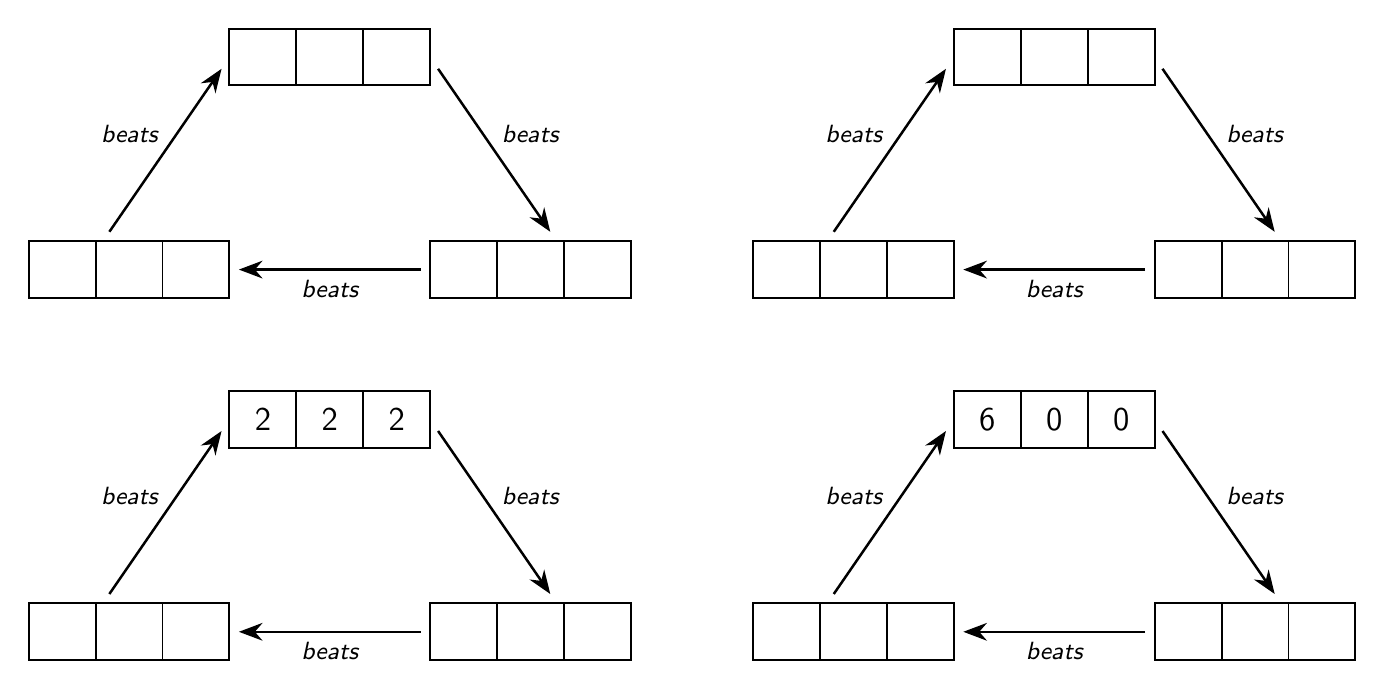
\begin{tikzpicture}[]
\draw[line width=0.7pt] (2.825,0.990) rectangle (3.675,1.710);
\draw[line width=0.7pt] (3.675,0.990) rectangle (4.525,1.710);
\draw[line width=0.7pt] (4.525,0.990) rectangle (5.375,1.710);
\draw[line width=0.7pt] (5.375,-1.710) rectangle (6.225,-0.990);
\draw[line width=0.7pt] (6.225,-1.710) rectangle (7.075,-0.990);
\draw[line width=0.7pt] (7.075,-1.710) rectangle (7.925,-0.990);
\draw[line width=0.7pt] (0.275,-1.710) rectangle (1.125,-0.990);
\draw[line width=0.7pt] (1.125,-1.710) rectangle (1.975,-0.990);
\draw[line width=0.7pt] (1.975,-1.710) rectangle (2.825,-0.990);
\draw[-{Stealth[length=3mm]},line width=0.9pt] (5.475,1.200) -- (6.900,-0.870) node[midway,above right=-1pt,font=\small\itshape] {beats};
\draw[-{Stealth[length=3mm]},line width=0.9pt] (5.255,-1.350) -- (2.945,-1.350) node[midway,below,font=\small\itshape] {beats};
\draw[-{Stealth[length=3mm]},line width=0.9pt] (1.300,-0.870) -- (2.725,1.200) node[midway,above left=-1pt,font=\small\itshape] {beats};
\draw[line width=0.7pt] (12.025,0.990) rectangle (12.875,1.710);
\draw[line width=0.7pt] (12.875,0.990) rectangle (13.725,1.710);
\draw[line width=0.7pt] (13.725,0.990) rectangle (14.575,1.710);
\draw[line width=0.7pt] (14.575,-1.710) rectangle (15.425,-0.990);
\draw[line width=0.7pt] (15.425,-1.710) rectangle (16.275,-0.990);
\draw[line width=0.7pt] (16.275,-1.710) rectangle (17.125,-0.990);
\draw[line width=0.7pt] (9.475,-1.710) rectangle (10.325,-0.990);
\draw[line width=0.7pt] (10.325,-1.710) rectangle (11.175,-0.990);
\draw[line width=0.7pt] (11.175,-1.710) rectangle (12.025,-0.990);
\draw[-{Stealth[length=3mm]},line width=0.9pt] (14.675,1.200) -- (16.100,-0.870) node[midway,above right=-1pt,font=\small\itshape] {beats};
\draw[-{Stealth[length=3mm]},line width=0.9pt] (14.455,-1.350) -- (12.145,-1.350) node[midway,below,font=\small\itshape] {beats};
\draw[-{Stealth[length=3mm]},line width=0.9pt] (10.500,-0.870) -- (11.925,1.200) node[midway,above left=-1pt,font=\small\itshape] {beats};
\draw[line width=0.7pt] (2.825,-3.610) rectangle (3.675,-2.890);
\node[font=\large] at (3.250,-3.250) {2};
\draw[line width=0.7pt] (3.675,-3.610) rectangle (4.525,-2.890);
\node[font=\large] at (4.100,-3.250) {2};
\draw[line width=0.7pt] (4.525,-3.610) rectangle (5.375,-2.890);
\node[font=\large] at (4.950,-3.250) {2};
\draw[line width=0.7pt] (5.375,-6.310) rectangle (6.225,-5.590);
\draw[line width=0.7pt] (6.225,-6.310) rectangle (7.075,-5.590);
\draw[line width=0.7pt] (7.075,-6.310) rectangle (7.925,-5.590);
\draw[line width=0.7pt] (0.275,-6.310) rectangle (1.125,-5.590);
\draw[line width=0.7pt] (1.125,-6.310) rectangle (1.975,-5.590);
\draw[line width=0.7pt] (1.975,-6.310) rectangle (2.825,-5.590);
\draw[-{Stealth[length=3mm]},line width=0.9pt] (5.475,-3.400) -- (6.900,-5.470) node[midway,above right=-1pt,font=\small\itshape] {beats};
\draw[-{Stealth[length=3mm]},line width=0.9pt] (5.255,-5.950) -- (2.945,-5.950) node[midway,below,font=\small\itshape] {beats};
\draw[-{Stealth[length=3mm]},line width=0.9pt] (1.300,-5.470) -- (2.725,-3.400) node[midway,above left=-1pt,font=\small\itshape] {beats};
\draw[line width=0.7pt] (12.025,-3.610) rectangle (12.875,-2.890);
\node[font=\large] at (12.450,-3.250) {6};
\draw[line width=0.7pt] (12.875,-3.610) rectangle (13.725,-2.890);
\node[font=\large] at (13.300,-3.250) {0};
\draw[line width=0.7pt] (13.725,-3.610) rectangle (14.575,-2.890);
\node[font=\large] at (14.150,-3.250) {0};
\draw[line width=0.7pt] (14.575,-6.310) rectangle (15.425,-5.590);
\draw[line width=0.7pt] (15.425,-6.310) rectangle (16.275,-5.590);
\draw[line width=0.7pt] (16.275,-6.310) rectangle (17.125,-5.590);
\draw[line width=0.7pt] (9.475,-6.310) rectangle (10.325,-5.590);
\draw[line width=0.7pt] (10.325,-6.310) rectangle (11.175,-5.590);
\draw[line width=0.7pt] (11.175,-6.310) rectangle (12.025,-5.590);
\draw[-{Stealth[length=3mm]},line width=0.9pt] (14.675,-3.400) -- (16.100,-5.470) node[midway,above right=-1pt,font=\small\itshape] {beats};
\draw[-{Stealth[length=3mm]},line width=0.9pt] (14.455,-5.950) -- (12.145,-5.950) node[midway,below,font=\small\itshape] {beats};
\draw[-{Stealth[length=3mm]},line width=0.9pt] (10.500,-5.470) -- (11.925,-3.400) node[midway,above left=-1pt,font=\small\itshape] {beats};
\end{tikzpicture}
\par\vspace{6pt}\par\noindent
\begin{tikzpicture}\draw[black!30,line width=0.5pt] (0,-0.850) -- (\linewidth-1pt,-0.850);\draw[black!30,line width=0.5pt] (0,-1.700) -- (\linewidth-1pt,-1.700);\draw[black!30,line width=0.5pt] (0,-2.550) -- (\linewidth-1pt,-2.550);\draw[black!30,line width=0.5pt] (0,-3.400) -- (\linewidth-1pt,-3.400);\draw[black!30,line width=0.5pt] (0,-4.250) -- (\linewidth-1pt,-4.250);\draw[black!30,line width=0.5pt] (0,-5.100) -- (\linewidth-1pt,-5.100);\end{tikzpicture}\par
\newpage
\prob{6}Find every plan with 6 cubes that beats \strip{2}{2}{2}, and explain how you know there are no others. Then find every plan with 6 cubes that beats \strip{6}{0}{0}.
\par\vspace{14pt}\noindent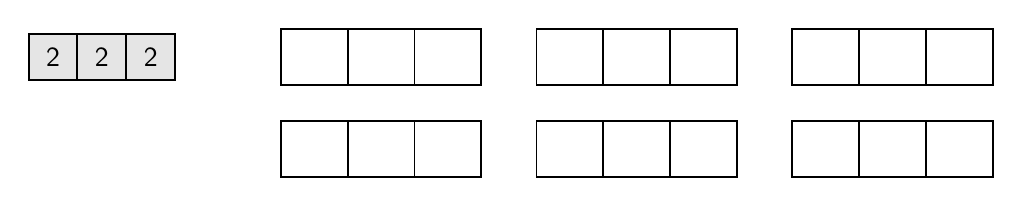
\begin{tikzpicture}[]
\draw[line width=0.7pt,fill=black!10] (0.000,0.000) rectangle (0.620,0.580);
\node[font=\normalsize] at (0.310,0.290) {2};
\draw[line width=0.7pt,fill=black!10] (0.620,0.000) rectangle (1.240,0.580);
\node[font=\normalsize] at (0.930,0.290) {2};
\draw[line width=0.7pt,fill=black!10] (1.240,0.000) rectangle (1.860,0.580);
\node[font=\normalsize] at (1.550,0.290) {2};
\draw[line width=0.7pt] (3.200,-0.070) rectangle (4.050,0.650);
\draw[line width=0.7pt] (4.050,-0.070) rectangle (4.900,0.650);
\draw[line width=0.7pt] (4.900,-0.070) rectangle (5.750,0.650);
\draw[line width=0.7pt] (6.450,-0.070) rectangle (7.300,0.650);
\draw[line width=0.7pt] (7.300,-0.070) rectangle (8.150,0.650);
\draw[line width=0.7pt] (8.150,-0.070) rectangle (9.000,0.650);
\draw[line width=0.7pt] (9.700,-0.070) rectangle (10.550,0.650);
\draw[line width=0.7pt] (10.550,-0.070) rectangle (11.400,0.650);
\draw[line width=0.7pt] (11.400,-0.070) rectangle (12.250,0.650);
\draw[line width=0.7pt] (3.200,-1.240) rectangle (4.050,-0.520);
\draw[line width=0.7pt] (4.050,-1.240) rectangle (4.900,-0.520);
\draw[line width=0.7pt] (4.900,-1.240) rectangle (5.750,-0.520);
\draw[line width=0.7pt] (6.450,-1.240) rectangle (7.300,-0.520);
\draw[line width=0.7pt] (7.300,-1.240) rectangle (8.150,-0.520);
\draw[line width=0.7pt] (8.150,-1.240) rectangle (9.000,-0.520);
\draw[line width=0.7pt] (9.700,-1.240) rectangle (10.550,-0.520);
\draw[line width=0.7pt] (10.550,-1.240) rectangle (11.400,-0.520);
\draw[line width=0.7pt] (11.400,-1.240) rectangle (12.250,-0.520);
\end{tikzpicture}
\par\vspace{2pt}\par\noindent\begin{tikzpicture}\draw[black!30,line width=0.5pt] (0,-0.850) -- (\linewidth-1pt,-0.850);\draw[black!30,line width=0.5pt] (0,-1.700) -- (\linewidth-1pt,-1.700);\draw[black!30,line width=0.5pt] (0,-2.550) -- (\linewidth-1pt,-2.550);\draw[black!30,line width=0.5pt] (0,-3.400) -- (\linewidth-1pt,-3.400);\end{tikzpicture}\par
\par\vspace{20pt}\noindent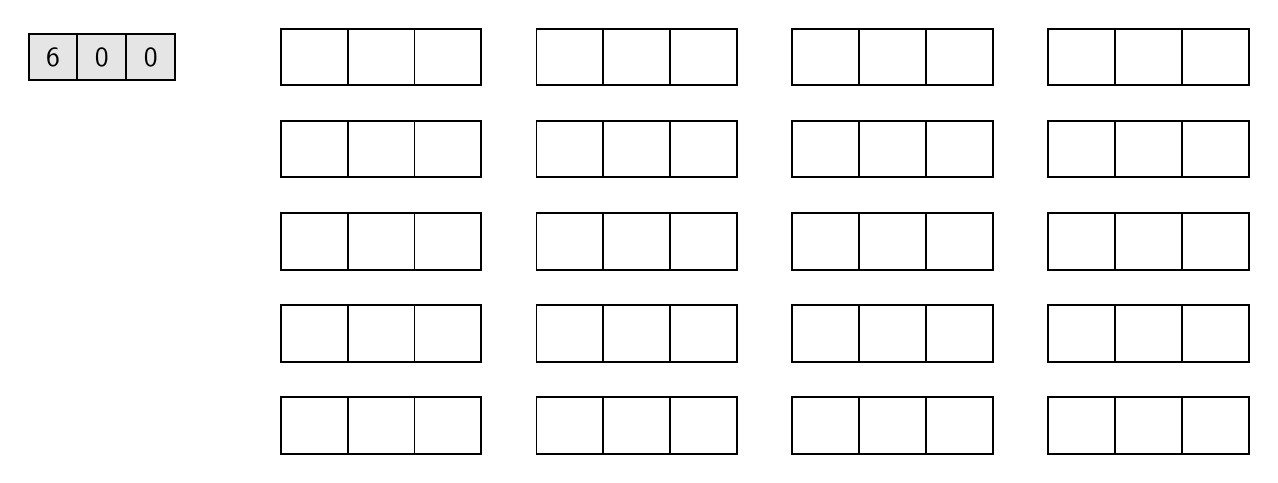
\begin{tikzpicture}[]
\draw[line width=0.7pt,fill=black!10] (0.000,0.000) rectangle (0.620,0.580);
\node[font=\normalsize] at (0.310,0.290) {6};
\draw[line width=0.7pt,fill=black!10] (0.620,0.000) rectangle (1.240,0.580);
\node[font=\normalsize] at (0.930,0.290) {0};
\draw[line width=0.7pt,fill=black!10] (1.240,0.000) rectangle (1.860,0.580);
\node[font=\normalsize] at (1.550,0.290) {0};
\draw[line width=0.7pt] (3.200,-0.070) rectangle (4.050,0.650);
\draw[line width=0.7pt] (4.050,-0.070) rectangle (4.900,0.650);
\draw[line width=0.7pt] (4.900,-0.070) rectangle (5.750,0.650);
\draw[line width=0.7pt] (6.450,-0.070) rectangle (7.300,0.650);
\draw[line width=0.7pt] (7.300,-0.070) rectangle (8.150,0.650);
\draw[line width=0.7pt] (8.150,-0.070) rectangle (9.000,0.650);
\draw[line width=0.7pt] (9.700,-0.070) rectangle (10.550,0.650);
\draw[line width=0.7pt] (10.550,-0.070) rectangle (11.400,0.650);
\draw[line width=0.7pt] (11.400,-0.070) rectangle (12.250,0.650);
\draw[line width=0.7pt] (12.950,-0.070) rectangle (13.800,0.650);
\draw[line width=0.7pt] (13.800,-0.070) rectangle (14.650,0.650);
\draw[line width=0.7pt] (14.650,-0.070) rectangle (15.500,0.650);
\draw[line width=0.7pt] (3.200,-1.240) rectangle (4.050,-0.520);
\draw[line width=0.7pt] (4.050,-1.240) rectangle (4.900,-0.520);
\draw[line width=0.7pt] (4.900,-1.240) rectangle (5.750,-0.520);
\draw[line width=0.7pt] (6.450,-1.240) rectangle (7.300,-0.520);
\draw[line width=0.7pt] (7.300,-1.240) rectangle (8.150,-0.520);
\draw[line width=0.7pt] (8.150,-1.240) rectangle (9.000,-0.520);
\draw[line width=0.7pt] (9.700,-1.240) rectangle (10.550,-0.520);
\draw[line width=0.7pt] (10.550,-1.240) rectangle (11.400,-0.520);
\draw[line width=0.7pt] (11.400,-1.240) rectangle (12.250,-0.520);
\draw[line width=0.7pt] (12.950,-1.240) rectangle (13.800,-0.520);
\draw[line width=0.7pt] (13.800,-1.240) rectangle (14.650,-0.520);
\draw[line width=0.7pt] (14.650,-1.240) rectangle (15.500,-0.520);
\draw[line width=0.7pt] (3.200,-2.410) rectangle (4.050,-1.690);
\draw[line width=0.7pt] (4.050,-2.410) rectangle (4.900,-1.690);
\draw[line width=0.7pt] (4.900,-2.410) rectangle (5.750,-1.690);
\draw[line width=0.7pt] (6.450,-2.410) rectangle (7.300,-1.690);
\draw[line width=0.7pt] (7.300,-2.410) rectangle (8.150,-1.690);
\draw[line width=0.7pt] (8.150,-2.410) rectangle (9.000,-1.690);
\draw[line width=0.7pt] (9.700,-2.410) rectangle (10.550,-1.690);
\draw[line width=0.7pt] (10.550,-2.410) rectangle (11.400,-1.690);
\draw[line width=0.7pt] (11.400,-2.410) rectangle (12.250,-1.690);
\draw[line width=0.7pt] (12.950,-2.410) rectangle (13.800,-1.690);
\draw[line width=0.7pt] (13.800,-2.410) rectangle (14.650,-1.690);
\draw[line width=0.7pt] (14.650,-2.410) rectangle (15.500,-1.690);
\draw[line width=0.7pt] (3.200,-3.580) rectangle (4.050,-2.860);
\draw[line width=0.7pt] (4.050,-3.580) rectangle (4.900,-2.860);
\draw[line width=0.7pt] (4.900,-3.580) rectangle (5.750,-2.860);
\draw[line width=0.7pt] (6.450,-3.580) rectangle (7.300,-2.860);
\draw[line width=0.7pt] (7.300,-3.580) rectangle (8.150,-2.860);
\draw[line width=0.7pt] (8.150,-3.580) rectangle (9.000,-2.860);
\draw[line width=0.7pt] (9.700,-3.580) rectangle (10.550,-2.860);
\draw[line width=0.7pt] (10.550,-3.580) rectangle (11.400,-2.860);
\draw[line width=0.7pt] (11.400,-3.580) rectangle (12.250,-2.860);
\draw[line width=0.7pt] (12.950,-3.580) rectangle (13.800,-2.860);
\draw[line width=0.7pt] (13.800,-3.580) rectangle (14.650,-2.860);
\draw[line width=0.7pt] (14.650,-3.580) rectangle (15.500,-2.860);
\draw[line width=0.7pt] (3.200,-4.750) rectangle (4.050,-4.030);
\draw[line width=0.7pt] (4.050,-4.750) rectangle (4.900,-4.030);
\draw[line width=0.7pt] (4.900,-4.750) rectangle (5.750,-4.030);
\draw[line width=0.7pt] (6.450,-4.750) rectangle (7.300,-4.030);
\draw[line width=0.7pt] (7.300,-4.750) rectangle (8.150,-4.030);
\draw[line width=0.7pt] (8.150,-4.750) rectangle (9.000,-4.030);
\draw[line width=0.7pt] (9.700,-4.750) rectangle (10.550,-4.030);
\draw[line width=0.7pt] (10.550,-4.750) rectangle (11.400,-4.030);
\draw[line width=0.7pt] (11.400,-4.750) rectangle (12.250,-4.030);
\draw[line width=0.7pt] (12.950,-4.750) rectangle (13.800,-4.030);
\draw[line width=0.7pt] (13.800,-4.750) rectangle (14.650,-4.030);
\draw[line width=0.7pt] (14.650,-4.750) rectangle (15.500,-4.030);
\end{tikzpicture}
\newpage
\prob{7}Now the two players may have different numbers of cubes. Beat each plan below with as few cubes as you can. Then find a quick way to tell how many cubes you need to beat any plan.
\par\vspace{12pt}\noindent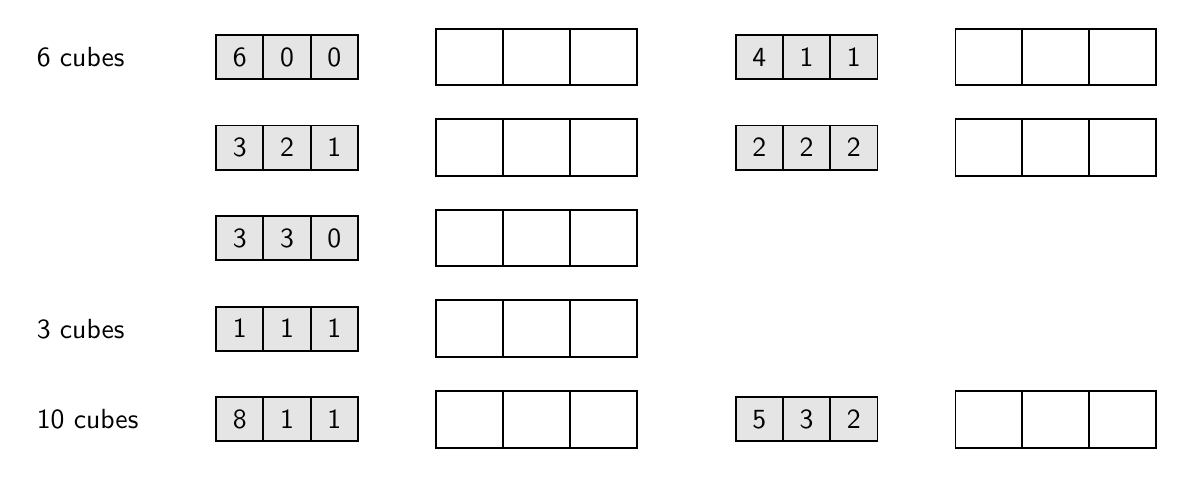
\begin{tikzpicture}[]
\node[anchor=west,font=\normalsize] at (0,0.360) {6 cubes};
\draw[line width=0.7pt,fill=black!10] (2.400,0.080) rectangle (3.000,0.640);
\node[font=\normalsize] at (2.700,0.360) {6};
\draw[line width=0.7pt,fill=black!10] (3.000,0.080) rectangle (3.600,0.640);
\node[font=\normalsize] at (3.300,0.360) {0};
\draw[line width=0.7pt,fill=black!10] (3.600,0.080) rectangle (4.200,0.640);
\node[font=\normalsize] at (3.900,0.360) {0};
\draw[line width=0.7pt] (5.190,0.000) rectangle (6.040,0.720);
\draw[line width=0.7pt] (6.040,0.000) rectangle (6.890,0.720);
\draw[line width=0.7pt] (6.890,0.000) rectangle (7.740,0.720);
\draw[line width=0.7pt,fill=black!10] (9.000,0.080) rectangle (9.600,0.640);
\node[font=\normalsize] at (9.300,0.360) {4};
\draw[line width=0.7pt,fill=black!10] (9.600,0.080) rectangle (10.200,0.640);
\node[font=\normalsize] at (9.900,0.360) {1};
\draw[line width=0.7pt,fill=black!10] (10.200,0.080) rectangle (10.800,0.640);
\node[font=\normalsize] at (10.500,0.360) {1};
\draw[line width=0.7pt] (11.790,0.000) rectangle (12.640,0.720);
\draw[line width=0.7pt] (12.640,0.000) rectangle (13.490,0.720);
\draw[line width=0.7pt] (13.490,0.000) rectangle (14.340,0.720);
\draw[line width=0.7pt,fill=black!10] (2.400,-1.070) rectangle (3.000,-0.510);
\node[font=\normalsize] at (2.700,-0.790) {3};
\draw[line width=0.7pt,fill=black!10] (3.000,-1.070) rectangle (3.600,-0.510);
\node[font=\normalsize] at (3.300,-0.790) {2};
\draw[line width=0.7pt,fill=black!10] (3.600,-1.070) rectangle (4.200,-0.510);
\node[font=\normalsize] at (3.900,-0.790) {1};
\draw[line width=0.7pt] (5.190,-1.150) rectangle (6.040,-0.430);
\draw[line width=0.7pt] (6.040,-1.150) rectangle (6.890,-0.430);
\draw[line width=0.7pt] (6.890,-1.150) rectangle (7.740,-0.430);
\draw[line width=0.7pt,fill=black!10] (9.000,-1.070) rectangle (9.600,-0.510);
\node[font=\normalsize] at (9.300,-0.790) {2};
\draw[line width=0.7pt,fill=black!10] (9.600,-1.070) rectangle (10.200,-0.510);
\node[font=\normalsize] at (9.900,-0.790) {2};
\draw[line width=0.7pt,fill=black!10] (10.200,-1.070) rectangle (10.800,-0.510);
\node[font=\normalsize] at (10.500,-0.790) {2};
\draw[line width=0.7pt] (11.790,-1.150) rectangle (12.640,-0.430);
\draw[line width=0.7pt] (12.640,-1.150) rectangle (13.490,-0.430);
\draw[line width=0.7pt] (13.490,-1.150) rectangle (14.340,-0.430);
\draw[line width=0.7pt,fill=black!10] (2.400,-2.220) rectangle (3.000,-1.660);
\node[font=\normalsize] at (2.700,-1.940) {3};
\draw[line width=0.7pt,fill=black!10] (3.000,-2.220) rectangle (3.600,-1.660);
\node[font=\normalsize] at (3.300,-1.940) {3};
\draw[line width=0.7pt,fill=black!10] (3.600,-2.220) rectangle (4.200,-1.660);
\node[font=\normalsize] at (3.900,-1.940) {0};
\draw[line width=0.7pt] (5.190,-2.300) rectangle (6.040,-1.580);
\draw[line width=0.7pt] (6.040,-2.300) rectangle (6.890,-1.580);
\draw[line width=0.7pt] (6.890,-2.300) rectangle (7.740,-1.580);
\node[anchor=west,font=\normalsize] at (0,-3.090) {3 cubes};
\draw[line width=0.7pt,fill=black!10] (2.400,-3.370) rectangle (3.000,-2.810);
\node[font=\normalsize] at (2.700,-3.090) {1};
\draw[line width=0.7pt,fill=black!10] (3.000,-3.370) rectangle (3.600,-2.810);
\node[font=\normalsize] at (3.300,-3.090) {1};
\draw[line width=0.7pt,fill=black!10] (3.600,-3.370) rectangle (4.200,-2.810);
\node[font=\normalsize] at (3.900,-3.090) {1};
\draw[line width=0.7pt] (5.190,-3.450) rectangle (6.040,-2.730);
\draw[line width=0.7pt] (6.040,-3.450) rectangle (6.890,-2.730);
\draw[line width=0.7pt] (6.890,-3.450) rectangle (7.740,-2.730);
\node[anchor=west,font=\normalsize] at (0,-4.240) {10 cubes};
\draw[line width=0.7pt,fill=black!10] (2.400,-4.520) rectangle (3.000,-3.960);
\node[font=\normalsize] at (2.700,-4.240) {8};
\draw[line width=0.7pt,fill=black!10] (3.000,-4.520) rectangle (3.600,-3.960);
\node[font=\normalsize] at (3.300,-4.240) {1};
\draw[line width=0.7pt,fill=black!10] (3.600,-4.520) rectangle (4.200,-3.960);
\node[font=\normalsize] at (3.900,-4.240) {1};
\draw[line width=0.7pt] (5.190,-4.600) rectangle (6.040,-3.880);
\draw[line width=0.7pt] (6.040,-4.600) rectangle (6.890,-3.880);
\draw[line width=0.7pt] (6.890,-4.600) rectangle (7.740,-3.880);
\draw[line width=0.7pt,fill=black!10] (9.000,-4.520) rectangle (9.600,-3.960);
\node[font=\normalsize] at (9.300,-4.240) {5};
\draw[line width=0.7pt,fill=black!10] (9.600,-4.520) rectangle (10.200,-3.960);
\node[font=\normalsize] at (9.900,-4.240) {3};
\draw[line width=0.7pt,fill=black!10] (10.200,-4.520) rectangle (10.800,-3.960);
\node[font=\normalsize] at (10.500,-4.240) {2};
\draw[line width=0.7pt] (11.790,-4.600) rectangle (12.640,-3.880);
\draw[line width=0.7pt] (12.640,-4.600) rectangle (13.490,-3.880);
\draw[line width=0.7pt] (13.490,-4.600) rectangle (14.340,-3.880);
\end{tikzpicture}
\par\vspace{10pt}\par\noindent
\begin{tikzpicture}\draw[black!30,line width=0.5pt] (0,-0.850) -- (\linewidth-1pt,-0.850);\draw[black!30,line width=0.5pt] (0,-1.700) -- (\linewidth-1pt,-1.700);\draw[black!30,line width=0.5pt] (0,-2.550) -- (\linewidth-1pt,-2.550);\draw[black!30,line width=0.5pt] (0,-3.400) -- (\linewidth-1pt,-3.400);\draw[black!30,line width=0.5pt] (0,-4.250) -- (\linewidth-1pt,-4.250);\draw[black!30,line width=0.5pt] (0,-5.100) -- (\linewidth-1pt,-5.100);\draw[black!30,line width=0.5pt] (0,-5.950) -- (\linewidth-1pt,-5.950);\draw[black!30,line width=0.5pt] (0,-6.800) -- (\linewidth-1pt,-6.800);\end{tikzpicture}\par

\end{document}
